%% -*- coding: utf-8 -*-
\documentclass[12pt,pagesize,paper=192mm:108mm,landscape]{scrbook} 
%1920x1080 1280x720
\areaset[current]{192mm}{108mm}
\usepackage{calc}
\usepackage[T2A]{fontenc}
\usepackage[utf8]{inputenc}
\usepackage[english,russian]{babel}
\usepackage{microtype}
\usepackage{misccorr}
\usepackage{cmap}
%\usepackage[unicode=true]{hyperref}
\usepackage{graphicx}
\usepackage{amssymb}
\usepackage{amsmath}
%\usepackage{srcltx}
\usepackage{textcomp}
\usepackage{xspace}
%научные символы и смайлики \smiley \frownie
\usepackage{wasysym}
\usepackage{ccicons}
\begin{document}
\begin{titlepage}
  \vspace*{-0.5em}
  \begin{center}    
    % \hspace*{3em}
    % \begin{minipage}[t]{3em}
    %   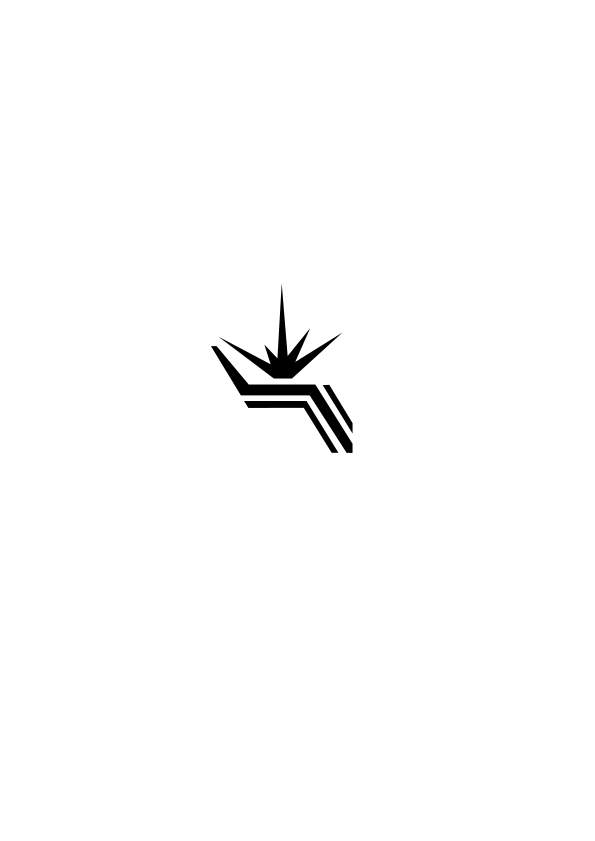
\includegraphics[width=\textwidth]{../BINP-logo}
    % \end{minipage}\hfill
    % \begin{minipage}{0.23\linewidth}
    % 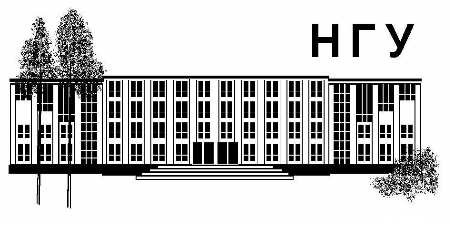
\includegraphics[width=\textwidth]{../NSU-logo}
    % \end{minipage}
    % \hfill
    % \hspace*{6em}

    
    % Кафедра теоретической физики физического факультета НГУ
    % \medskip

    % \Large
    % Профессор Грабовский А.\,В.
    % \smallskip

    % \huge
    % \textbf{Общая теория относительности}
    % \smallskip

    % \Large
    % Лекция № 10
     \vfill

     \normalsize
     \begin{minipage}{0.9\linewidth}
      Теорема Фробениуса. Доказательство постоянства поверхностной
      гравитации на орбитах вектора Киллинга на горизонте
      Киллинга. Невырожденный горизонт Киллинга. Доказательство того,
      что если на орбите вектора Киллинга на горизонте Киллинга
      поверхностная гравитация не равна 0, то эта орбита является
      частью нулевого генератора горизонта Киллинга. Точка
      бифуркации. Доказательство постоянства квадрата поверхностной
      гравитации на~горизонте Киллинга. Вычисление поверхностной
      гравитации на~горизонте Киллинга в поле Шварцшильда в
      координатах Крускала. Пространство время Риндлера как
      пространство время Шварцшильда вблизи горизонта. Горизонт и
      поверхностная гравитация в~пространстве времени
      Риндлера. Вычисление собственного ускорения частицы с
      координатой $х$ в пространстве Риндлера.
    \end{minipage}
    \vfill

    \normalsize \ccbysa\hspace{0.5em}  Новосибирск 2022
  \end{center}
\end{titlepage}
\end{document}
